%% Preambel
\documentclass[conference,compsoc,final,a4paper]{IEEEtran}
\usepackage[utf8]{inputenx}

%% Bitte legen Sie hier den Titel und den Autor der Arbeit fest
\newcommand{\autoren}[0]{Cöllen, Markus}
\newcommand{\dokumententitel}[0]{Kann Malware in Android-Apps automatisch gefunden
werden?}

% Hie muss normalerweise nichts angepasst werden
\usepackage[pdftex]{graphicx}
\graphicspath{{img/}}
\DeclareGraphicsExtensions{.pdf,.jpeg,.jpg,.png}
\usepackage[cmex10]{amsmath}
\usepackage{algorithmic}
\usepackage{array}
\usepackage{dblfloatfix}
\usepackage{url}
\usepackage[autostyle=true,german=quotes]{csquotes}
\usepackage[backend=bibtex]{biblatex}
\usepackage{booktabs}
\usepackage{xcolor}
\usepackage{listings}             % Source Code listings
\usepackage[printonlyused]{acronym}

% Farben definieren
\definecolor{linkblue}{RGB}{0, 0, 100}
\definecolor{linkblack}{RGB}{0, 0, 0}
\definecolor{darkgreen}{RGB}{14, 144, 102}
\definecolor{darkblue}{RGB}{0,0,168}
\definecolor{darkred}{RGB}{128,0,0}
\definecolor{comment}{RGB}{63, 127, 95}
\definecolor{javadoccomment}{RGB}{63, 95, 191}
\definecolor{keyword}{RGB}{108, 0, 67}
\definecolor{type}{RGB}{0, 0, 0}
\definecolor{method}{RGB}{0, 0, 0}
\definecolor{variable}{RGB}{0, 0, 0}
\definecolor{literal}{RGB}{31,0, 255}
\definecolor{operator}{RGB}{0, 0, 0}

\usepackage[ngerman]{betababel}
\usepackage[
	    unicode=true,
      hypertexnames=false,
      colorlinks=true,
      colorlinks=false,
      linkcolor=darkblue,
      citecolor=darkblue,
      urlcolor=darkblue,
      pdftex
   ]{hyperref}
%	 \PrerenderUnicode{ü}

% Einstellungen für Quelltexte
\lstset{
      xleftmargin=0.1cm,
      basicstyle=\scriptsize\ttfamily,
      keywordstyle=\color{keyword},
      identifierstyle=\color{variable},
      commentstyle=\color{comment},
      stringstyle=\color{literal},
      tabsize=2,
      lineskip={2pt},
      columns=flexible,
      inputencoding=utf8,
      captionpos=b,
      breakautoindent=true,
	  breakindent=2em,
	  breaklines=true,
	  prebreak=,
	  postbreak=,
      numbers=none,
      numberstyle=\tiny,
      showspaces=false,      % Keine Leerzeichensymbole
      showtabs=false,        % Keine Tabsymbole
      showstringspaces=false,% Leerzeichen in Strings
      morecomment=[s][\color{javadoccomment}]{/**}{*/},
      literate={Ö}{{\"O}}1 {Ä}{{\"A}}1 {Ü}{{\"U}}1 {ß}{{\ss}}2 {ü}{{\"u}}1 {ä}{{\"a}}1 {ö}{{\"o}}1
}

\hypersetup{
  pdftitle={\dokumententitel},
	pdfauthor={\autoren},
	pdfdisplaydoctitle=true
}

% Wo liegt Sourcecode?
\newcommand{\srcloc}{src/}

% Literatur einbinden
\addbibresource{literatur.bib}

\begin{document}

% Titel des Dokuments
\title{\dokumententitel}

% Namen der Autoren
\author{
  \IEEEauthorblockN{\autoren}
  \IEEEauthorblockA{
    Hochschule Mannheim\\
    Fakultät für Informatik\\
    Paul-Wittsack-Str. 10,
    68163 Mannheim
    }
}

% Titel erzeugen
\maketitle
\thispagestyle{plain}
\pagestyle{plain}
 % Weitere Einstellungen aus einer anderen Datei lesen

% Eigentliches Dokument beginnt hier
% ----------------------------------------------------------------------------------------------------------

% Kurze Zusammenfassung des Dokuments
\begin{abstract}
An dieser Stelle steht eine kurze Zusammenfassung des Inhaltes des Dokuments.
\end{abstract}

\tableofcontents

\section{Einleitung}
Smartphones bieten aufgrund ihrer vielen Schittstellen zur Außenwelt, wie z.B. WLAN, Bluetooth, NFC, USB usw. viele Angriffspunkte. Ein Hauptgrund, warum Smartphones mit dem Android Betriebssystem so beliebt für Angreifer sind, ist der hohe Verbreitungsgrad dieser Geräte. Dieser liegt im Jahr 2018 bei ca. 86 Prozent und ist somit Sechs mal so hoch wie der Konkurrent IOS mit knapp 16 Prozent Marktanteil \cite{AndoidMarktanteil}.
Da Malware-Autoren immer mehr auf Verschleierungsmechanismen wie Komprimierung, Verschlüsselung oder sich selbst modifizierender Programmcode setzten, wird es für Antiviren Herstellern zunehmend schwieriger diese als schädliche Software zu erkennen \cite{Lehner2006}.

\section{Grundlagen}

\subsection{Was ist Android?}
Das Betriebssystem Android ist eine umfassende Open Source Plattform für Smartphones. Eigentümer des Android Betriebssystem ist die Open Handset Alliance, welches ein Konsortium von 84 Unternehmen ist, Ihr Ziel ist es "eine beschleunigte Innovation im Mobilbereich, um dem Benutzer ein reicheres, kostengünstigeres und besseres Mobilerlebnis zu bieten" \cite{gargenta2011einfuhrung}. Die Android Architektur besteht aus insgesamt fünf Schichten, dem Linux Kernel, Bibliotheken, Android-Laufzeitumgebung, Application-Frameworks und auf der obersten Schicht die Anwendungen. 

\begin{figure}[!ht]
\centering
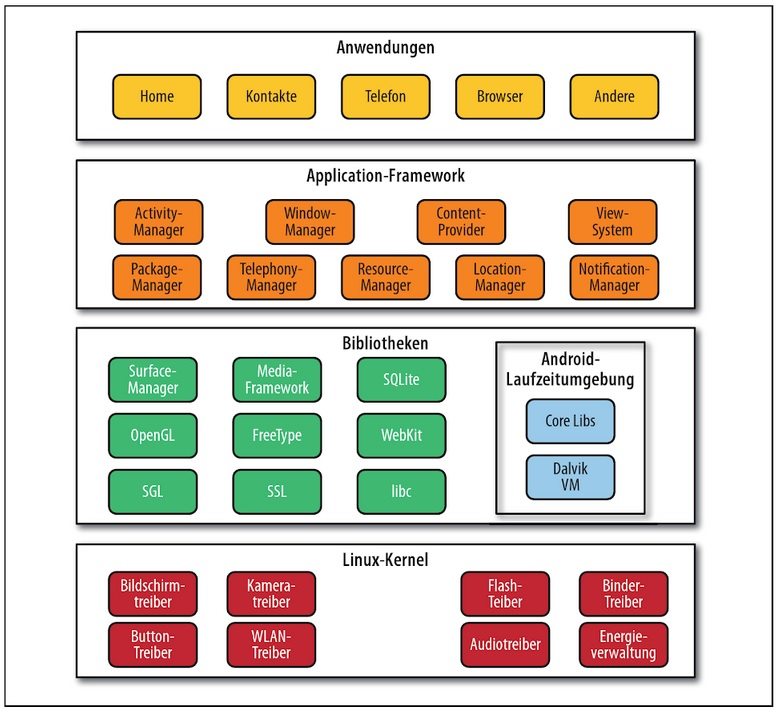
\includegraphics[width=8.5cm]{AndroidArchitektur}
\caption{Android Architektur ~\cite{gargenta2011einfuhrung}}
\label{fig_Android}
\end{figure}

Weil Android unter der Apache Open-Source Lizenz freigegeben ist und das Betriebssystem auf dem Linux-Kernel basiert, können Hersteller das Android Betriebssystem beliebig verwenden und für ihre Produkte anpassen. Zudem dient der Linux-Kernel als eine Abstraktion zwischen Software und Hardware und somit kann Android auf verschiedenen Geräten eingesetzt werden. Aufgrund der Tatsache, dass Linux über ein etabliertes Sicherheitskonzept verfügt \cite{LinuxSicherheitskonzept}, greift Android auf viele Schutzmechanismen des Linux Kernels zurück oder benutzt diese als ihre Basis\cite{scheid2012kapitel}. Zudem verwendet Android viele von Linux mitgebrachten Funktionen wie z.B. die Unterstüzung für Speicherverwaltung, Power-Management und Netzwerkzugriff. Wie man in Abbildung \ref{fig_Android} sehen kann, gibt es zudem noch viele von Android mitgebrachte Bibliotheken wie SQLite (eine SQL Datenbank) oder OpenGL (eine 3-D-Grafikbibliothek). Bis zu den Android Versionen 4.x war die Dalvik VM ein Hauptbestandteil des Android Betriebssystem. Hierdurch wurde die geschriebenen Apps erst in Bytecode formatiert wenn sie auch wirklich gebraucht werden. Ab Android 5.x wurde dies durch den Ahead-of-time-Compiler ersetzt. Dieser übersetzt die Apps schon beim installieren in Bytecode-Format. Hierdurch wird sich bessere Performance und eine Beschleunigung von Apps erhofft ohne dabei Flexibilität verzichten zu müssen\cite{Dalvik}. Die Schicht Application-Framework stellt einem Entwickler die unterschiedlichsten Dienste zur Verfügung. Hierzu zählen viele Dienste, welche für eine Applikation die Infrastruktur zur Verfügung stellt, wie die Positionsermittlung, Sensoren, WLAN oder Telefoniefunktionen. Diese Schicht ist  für die Programmierung von Android Apps die wichtigste und daher auch  am gründlichsten Dokumentiert. Die oberste Schichte sind die Anwendungen. Diese sind teilweise schon vorinstalliert oder können heruntergeladen und installiert werden.


\subsection{Android Update Problematik}\label{sec:Android Update Problematik}

Wie man in Abbildung \ref{fig_sim} sehen kann verdrängen die neueren Android Versionen die älteren. Allerdings ist Android Oreo, mit gerade mal 4,6 Prozent, eine der am wenigsten vertretenen Version, obwohl sie die neueste und auch schon seit dem 27. August 2017 auf dem Markt ist. 

\begin{figure}[!ht]
\centering
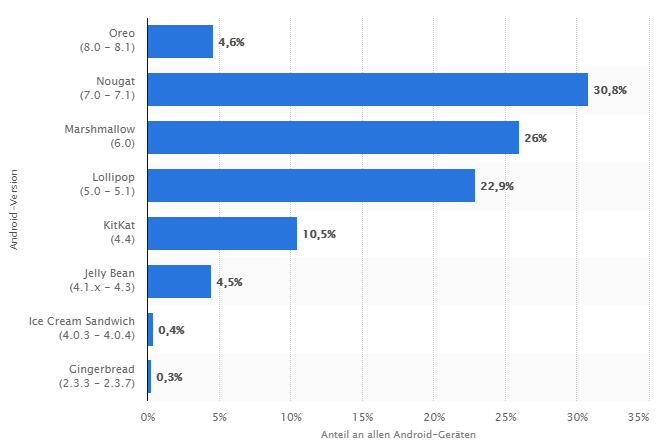
\includegraphics[width=8.5cm]{AndroidVersionen2}
\caption{Verteilung der Android-Versionen im Jahr 2018 ~\cite{Android-Versionen}}
\label{fig_sim}
\end{figure}

Dies liegt daran, dass nicht jede Android Version mit jedem Handy kompatibel ist. Die Smartphone Hersteller müssen die Versionen an ihre Geräte und die jeweilige Hardware anpassen. Diese umfassen Anpassungen an WLAN, Kamera, Bluetooth, GPS  usw. Anschließend müssen die erstellten Anpassungen noch umfangreich getestet werden, was auch noch viel Zeit in Anspruch nimmt. Weil die Hersteller oft neue Produkte verkaufen wollen und das Updaten älterer Smartphones zu teuer und zeitaufwendig ist, bleibt den Nutzern oft nichts anderes übrig, als neue Smartphones zu kaufen. Andernfalls behält man ein Smartphone mit einer veralteten Version und bekannten Sicherheitslücken. \cite{scheid2012kapitel}.  

\subsection{Application Sandbox}
\label{sec:Application Sandbox}
Linux arbeitet als ein Mehrbenutzer-Betriebssystem. Dies bedeutet, dass es mehrere Nutzer geben kann und das Betriebssystem verhindert, dass Daten eines Nutzers von einem anderen Nutzer eingesehen, geändert oder gelöscht werden können. Diese Nutzermanagement wird beim Application Sandboxing verwendet. Hierbei erhält jede Applikation eine eigene Nutzer-ID und führt diese in einem separaten Prozess aus. Somit gewährleistet Android, dass eine Applikation anderen Applikationen oder dem Betriebssystem keinen Schaden zufügen kann. Sollte eine Applikation aber durch das Ausnutzen einer Schwachstelle oder einer Sicherheitslücke an Root-Rechte kommen, kann die Applikation dieses Application Sandboxing einfach umgehen. Wie schon in Abschnitt \ref{sec:Android Update Problematik} beschrieben, gibt es wegen den stark verzögerten Android Updates oft Sicherheitslücken, welche über längere Zeit bekannt sind und leicht ausgenutzt werden können um Root-Rechte zu erlangen \cite{gargenta2011einfuhrung}.

\subsection{Permission Model}
\label{sec:Permission Model}
Standardmäßig hat eine Applikation keinen Zugriff auf Daten außerhalb der Sandbox. Sollte eine Applikation Systemressourcen außerhalb dieser verwenden wollen, muss erst eine Zugriffsanfrage gestellt werden. Geschützte Ressourcen sind z.B. Kamera, SMS, Bluetooth usw. \cite{PermissonModel}. Diese Rechte können bei einer Anfrage allerdings nur angenommen oder abgelehnt werden, bestimmte Einschränkungen können also nicht vorgenommen werden. Hier sollte der Nutzer sich Gedanken darüber machen, welche Applikationen welche Systemressourcen wirklich benötigen. Sollte ein Spiel wie z.B. Snake Rechte anfordern SMS zu verschicken, könnte dem Nutzer klar werden, dass etwas mit der Applikation nicht stimmt.

\subsection{Sicherheit des Google Play Store}
Anders als bei IOS, bei welchem die Nutzer an den Apple Store gebunden sind, können die Android Benutzer selbst entscheiden welchen Store sie verwenden. Der Google Play Store ist mit 82 Milliarden Downloads  \cite{GooglePlayDownloads} mit Abstand die größte Plattform. Er wurde am 28. August 2008 unter dem Namen Android Market veröffentlicht. Dieser bietet den Nutzern einfaches herunterladen und installieren von mobilen Anwendungen, sogenannten Applikationen. Im Google Play Store sind inzwischen über 3,7 Millionen Anwendungen  bereit zum Herunterladen \cite{Apps} und jeden Monat kommen ca. 30.000 neue Applikationen hinzu \cite{bartsch2014zertifizierte}. Durch den rasanten Wachstum steigt auch die Anzahl von schädlicher Software, sogenannter Malware. Der Anteil von bösartigen Applikationen ist von 2011 bis 2013 um 388\% gewachsen \cite{RiskIQ}. Da nicht alle Anwendungen von Mitarbeitern geprüft werden können, hat Google das Programm Bouncer ins Leben gerufen (siehe Kapitel \ref{sec:Bouncer}).
Android bietet zudem die Möglichkeit per Remote-Verbindung Applikationen zu installieren und zu löschen. Hierfür braucht man lediglich Zugriff auf den Google Play Account. Falls ein Angreifer an diese Daten kommen sollte, könnte er ohne Erlaubnis des Nutzers, Applikationen aus dem Google Play Store auf dem Smartphone installieren.

\subsection{Malware} \label{sec:Malware}
Bei dem Begriff Malware handelt es sich um ein Kunstwort, welches sich aus malicous und software zusammensetzt und bezeichnet Programme, welche unerwünschte oder auch schädliche Funktionen ausführen. Maleware kann man prinzipiell in drei unterschiedliche Hauptkathegorien unterteillen, Viren, Würmer und Trojaner. Ein Virus ist eine Software, welche sich selbst vervielfälltigen kann. Durch das Ausführen einer Infizierten Anwendung wird das Programm gestartet und schleust sich in anderen Programmen oder Dokumenten ein. Die sogenannten Würmer haben ähnliche Eigenschaften wie Vieren, der Hauptunterschied liegt darin, dass sie sich über das Intra- order Internet vermehren können und oft keine Interaktion mit den betroffenen Benutzern benötigen. Die dritte und gefährlichste Kathegorie ist das sogenannte Trojanische Pferd. Dieses täuscht dem Nutzer ein nützliches Programm vor, führt allerdings ohne Wissen des Benutzers im Hintergrund schädliche Funktionen und Routinen durch. Allerdings enthält die meiste Malware mehr als nur eine schädliche Funktion, was eine eindeutige Klassifikation fast unmöglich macht. Weitere Arten sind zudem Spyware, Exploits, Backdoors und Rootkits. Jede dieser Arten kann von ihren Maleware-Authoren druch Verschleierungsmechanismen wie Komprimierung, Verschlüsselung oder sich selbst modifizierender Programmcode verschleiert werden, was das Auffinden durch Vierenprogramme um einiges erschwert. \cite{Lehner2006} Die erfolgreichsten und am meisten genutzten Arten sind dabei Code Obfuscation, Anti-Analyse, Laufzeitpacker, Polymorphie und Metamorphie. 

\textbf{Code Obfuscation} bezeichnet dabei die Transformation des Quellcodes mit dem Ziel, die Ermittlung der Semantik und der Funktionalität zu erschweren ohne dabei die eigentliche Funktionalität des Programmes zu verändern \cite{bierbaummalicious}. Hierzu werden zum Beispiel leere Berechnungen eingebaut, Funktionen in viele kleine Teile aufgespalten oder Befehlsabfolgen kompliziert Reorganisiert. 

\textbf{Anti-Analyse} beschreibt hingegen das torpedieren wichtiger Werkzeuge wie Disassembler, Debugger und Emulatoren welche für das erstellen von Control Flow-Graphen \ref{sec:Kontrollflussanalyse} gebraucht werden. 

\textbf{Laufzeitpacker} sind Programme, welche den Programmcode komprimieren. Dies kann man sich ähnlich wie bei einem ZIP-Archiv vorstellen. Dies hat zur Folge, dass bei Ansicht des Programmcodes nur der Code des Packers sichtbar ist und nicht der Code der eigentlich ausgeführt wird.\cite{Benzmueller2018} Die Entschlüsselung der sogenannten Payload geschieht durch einen Decrypter zur Laufzeit. 

\textbf{Polymorphie} hat die Bedeutung Vielgestaltigkeit. Sollte das Programm nun von einem Laufzeitpacker verschlüsselt worden sein aber nach jeder Replikation seinen Schlüssel zur Ver- und Entschlüsselung ändern, nennt man dies ein polymorphes Programm.
Dieses Verfahren wird in Abbildung \ref{fig_Decrypter} gezeigt.

\begin{figure}[!ht]
\centering
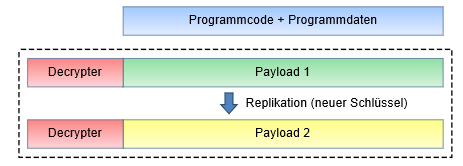
\includegraphics[width=8.5cm]{Decrypter}
\caption{Polymorphie des Programmcodes ~\cite{entpackermalware}}
\label{fig_Decrypter}
\end{figure}

\textbf{Metamorphie} hat die Bedeutung Verwandlung. Sollte nun nicht nur, wie in Abbildung \ref{fig_Decrypter} gezeigt ist, die Payload jedes mal geändert werden, sondern auch der Decrypter, spricht man von einem Methamorphosen Programm. Dies hat zur folge, dass der gesamte Quellcode nach jeder Replikation verändert ist. \cite{entpackermalware}
 
Malware stellt wegen all dieser Verschleierungsmechanismen eine immer größer werdende Bedrohung dar und durch den rasanten Wachstum des Smartphone-Marktes ist eine manuelle Auswertung mittlerweile unmöglich geworden. Obwohl es sich bei vielen neuen Arten um verschiedene Varianten bereits bekannter Malware handelt, müssen Analysten erst jedes Sample erneut analysieren um dies feststellen zu können \cite{trinius2010visualisierung}. Bei der Analyse kann grundsätzlich in zwei Arten unterschieden werden: Statische und Dynamische Analyse (siehe Kapitel \ref{sec:Statische Analyse} und \ref{sec:Dynamische Analyse}).

\section{Ansätze zur Merkmalsgenerierung}
\subsection{Dynamische Analyse} \label{sec:Dynamische Analyse}
Bei der dynamischen Analyse wird das Programm während der Laufzeit untersucht. Der Ablauf besteht dabei aus drei Teilen: der Ausführung des Programms, der Protokollierung des Ablaufes und der Ergebnisse und das Analysieren dieser \cite{dynamische_analyse}. Ein Beispiel der dynamischen Analysemethoden ist das Testen. Ein bedeutender Nachteil ist es, dass nicht immer alle Eingabeparameter überprüft werden können da diese exponentiell mit der Anzahl der Parameter steigt. Daher werden oft nur Rand- und Grenzfälle geprüft. Weitere Probleme können bei der Netzkommunikation, der Erstellung von Zufallszahlen wie auch bei Nutzereingaben auftreten. Wegen all dieser Eigenschaften eines Programmes ist eine Reproduzierbarkeit der Ergebnisse nicht gegeben. Zudem gibt es die Möglichkeit für Malware während Laufzeit zu erkennen, ob sie überprüft wird und kann sich gegebenenfalls zu diesem Zeitpunkt harmlos verhalten. Viele dieser Nachteile lassen sich durch eine statische Analyse vermeiden welche im  Abschnitt \ref{sec:Statische Analyse} vorgestellt wird.

\subsection{Statische Analyse} \label{sec:Statische Analyse}
Bei der statischen Analyse wird versucht durch reverse engineering Code aus der Maleware zu extrahieren um somit auf das Verhalten des Programmes schließen zu können. Dieser extrahierte Code kann anschließend eingehend untersucht werden. \cite{trinius2010visualisierung}. Diese Analysemethode wird also im Gegensatz zu dynamischen Analyse nicht zur Laufzeit des Programms angewandt und somit muss die App auch nicht ausgeführt werden. Da die korrekte Abbildung der Struktur des Quellcodes eine komplexe Aufgabe ist, wird hierzu oft ein Compiler verwendet. Dieser erzeugt aus dem Quellcode mit der Hilfe eines Lexers einen Tokenstream, also eine Folge aus den kleinsten sinntragenden Einheiten des Programms wie Literalen, Bezeichnern und Schlüsselwörtern, ein Beispiel hierfür wäre eine if-else Anweisung. Anschließend erzeugt ein Parser aus dem Tokenstream einen abstrakten Syntaxbaum, welcher die syntaktischen Zusammenhänge der einzelnen Tokens darstellt. Durch eine anschließende semantische Analyse wird aus dem Syntaxbaum ein Graph, auf welchen beispielsweise eine Kontrollflussanalyse\ref{sec:Kontrollflussanalyse} oder Datenflussanalyse \ref{sec:Datenflussanalyse} durchgeführt werden kann.

\subsubsection{Kontrollflussanalyse}\label{sec:Kontrollflussanalyse}
Bei der Kontrollflussanalyse wird untersucht, welcher Block im zu untersuchendem Programm
die Kontrolle an welchen Block übergibt, und welche Funktionen
dabei erreichbar sind. Zudem wird überprüft welche Werte Parameter einer Funktion möglicherweise zugewiesen bekommen. Um die Ergebnisse zu Analysieren wird ein Kontrollflussgraph erstellt. Dieser besteht aus einer Menge Knoten welche die Grundblöcke des Programmes darstellen. Zudem gibt es noch eine Menge von gerichteten Kanten, welche einen Übergang von einem Block zu einem anderen darstellen. Diese zeigen wie die Kontrolle von einem Block zu einem anderen übergeht. \cite{7365827} Die Abbildung \ref{fig_Kontrollflussgraph} zeigt ein Beispiel eines solchen Kontrollflussgraphen.

\begin{figure}[!ht]
\centering
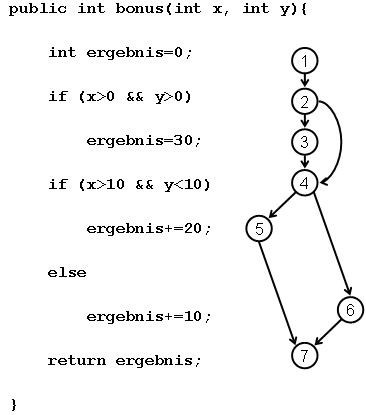
\includegraphics[width=6.5cm]{Kontrollflussgraph}
\caption{Kontrollflussgraph ~\cite{Kontrollflussgraph}}
\label{fig_Kontrollflussgraph}
\end{figure}

Wie man in Abbildung \ref{fig_Kontrollflussgraph} sehen kann, wird für jede Anweisung ein Block erstellt. int ergebnis=0; ist die erste Anweisung und somit auch Block 1. Block 2 ist die if Bedingung und je nachdem ob sie erfüllt wird geht sie zu Block 3, ergebnis=30; oder zur nächsten if Bedingung über. Bei dieser wird entweder der if Block oder der else Block ausgeführt, daher kommt auch die Verzweigung bei Block 4. return ergebnis; wird immer ausgeführt, daher laufen Block 5 und Block 6 auch in Block 7 wieder zusammen. Diese Kontrollflussgraphen werden auch zum überprüfen der Überdeckung verwendet.


\subsubsection{Datenflussanalyse}\label{sec:Datenflussanalyse}
Bei der Datenflussanalyse wird untersucht, welche Teiles des Programmes welche Daten weitergeben und welche Abhängigkeiten daraus resultieren. Als Grundlage dieser Methode wird ein Kontrollflussgraph aus Kapitel \ref{sec:Kontrollflussanalyse} verwendet. Die Datenflussanalyse untersucht, wie sich Daten durch die einzelnen Blöcke verändern. Enthält ein Block beispielsweise den Code x=1, so verändert sich der Wert von x nach dem Block auf 1. Diese gesamten Änderungen jedes Blocks werden überwacht und aufgezeichnet. \cite{7365827}

\subsection{Gegenüberstellung von statischer und dynamischer Analyse}
Durch eine dynamische Analyse können durch die Ausführung des Programmes konkrete Fehler gefunden werden, allerdings kann durch diese Methode nicht die Fehlerfreiheit des Programmes bewiesen werden, da das Programm meistens nicht mit allen Parametern gestartet und durchgeführt werden kann. Bei der statischen Analyse kann das Ausführen des Programmes mit allen möglichen Parametern betrachtet werden. Somit kann bewiesen werden, dass bestimmte Fehlerarten nicht auftreten können. Allerdings können Fehler auftreten welche durch das Fehlen entfernter Zusammenhänge entstehen. Zudem ist das Untersuchen mit dem statischen Ansatz Ungefährlich, da das Programm nicht laufen muss. Beide Analysemethoden haben Vor- und Nachteile, ergänzen sich allerdings gegenseitig gut, daher sollten beide Methoden zusammen verwendet werden. \cite{ernst2003static}

\section{Erkennungsmechanismen}

\subsection{signaturbasierte Malwareerkennung}
Die am meisten Vertretene Methode der Malwareerkennung ist die auf Signatur basierte Erkennung von Malware. Diese Methode basiert auf der statischen Analyse \ref{sec:Statische Analyse} und extrahiert aus einem potentiellen Malware-Programm eine eindeutige Byte-Folge , welche als eindeutige Identifikation und Signatur dient, und vergleicht diese mit allen verfügbaren Signaturen in der Erkennungssoftware Datenbank. Wird diese Signatur in einem anderen Programm gefunden, kann mit einer hohen Sicherheit davon ausgegangen werden, dass das Programm schädliche Komponenten enthält. Der erste große Nachteil dabei ist, dass nur bereits bekannte  Malwarearten gefunden werden können, zudem ist das Gerät in der gesamten Zeit in der die Signaturen verglichen werden gegen Angriffe ungeschützt. \cite{Lehner2006}





\subsection{Virenschutz durch Machine Learning}
Glaubt man den Firmen , welche Machine Learning für ihr Virenerkennung einsetzten, so hat die traditionelle Malwareerkennung ein Ende gefunden. Sobald man sich mit Machine Learning auseinander setzt wird man auch auf den Begriff Künstliche Intelligenz stoßen. Dieser ist ein Teil des Forschnungsgebietets der Informatik. Allerdings ist Intelligenz nur mangelhaft definiert und somit lässt sich dieses Forschnungsgebietet nur so einschränken, dass es sich nicht um eine Abarbeitung festgelegter Befehlssequenzen handelt. Die Berücksichtigung weitere Merkmale wie zum Beispiel Verarbeitung von Sprache, Visuelle Erkennung, Kreativität, Schlussfolgern und allgemeine Lernfähigkeit hängen von der Sicht des Benutzers ab. Das Lernen in Machine Learning impliziert dabei, dass Informationen Rückmeldung von Außerhalb dazu führen, dass eine Aufgabe besser gelöst werden kann. Dabei spielen folgende drei Kernaufgaben des Machine Learnings eine große Rolle. Erstens, eine Vorhersage treffen, zweitens Ursache finden und verstehen und drittens Muster in meistens nicht sortierten Daten erkennen. Umso mehr Daten in der sogenannten Lernphase eingespielt werden, desto sicherer und höher ist die Erkennungsrate. Virenschutzprogramme mit Machine Learning verwenden zwei Ansetzte, die statische \ref{sec:Statische Analyse} und die dynamische Analyse  \ref{sec:Dynamische Analyse}. In der statischen Analyse wird der Inhalt, also der Quellcode eines Programmes bewertet, ähnlich wie bei der signaturbasierten Malwareerkennung. Bei der dynamischen Analyse wertet das Virenprogramm während der Laufzeit Informationen über Prozesse, Interprozesskommunikation, Dateisystemzugriffe,  Muster in der Netzwerkkommunikation und Aktionen in der Registry aus. Der Virenschutz durch Machine Learning hat allerdings die selben Probleme wie andere Malwareerkennungsmethoden. Die Malware entzieht sich der Entdeckung durch verschiedene Verschleierungsmethoden, welche in Abschnitt \ref{sec:Malware} beschrieben wurden. Zudem können Neuronale Netze eine Aussage nur mit einer gewissen wahrscheinlichkeit ermöglichen, daher kann keine 100 \%ige Erkennung garantiert werden. \cite{Benzmueller2018}

\subsection{Integritätsprüfung}
Damit sich ein Virus verbreiten kann, muss er sich in andere Daten hineinkopieren und dabei Änderungen an dieser vornehmen. Ein Virenschutz kann diese Änderungen erkennen und somit auf eine Infizierung schließen. Dabei bildet der Virenschutz eine einmalige Checksumme über jede Datei des Systems und speichert diese in einer Datenbank. Sollte nun ein Virus eine Datei verändern ändert sich die Checksumme dieser Datei. Wir nun dieser unterschied einer Checksumme festgestellt kann mit einer hohen Sicherheit auf ein Virus geschlossen werden. Mit dieser Technik ist es möglich die Anwesenheit auch bisher unbekannte Malware festzustellen. Das große Problem ist dabei, dass nicht nur Malware, sondern auch der Nutzer, legale Programme oder auch Updates Daten auf dem System verändern können. Zudem wird die Malware erst bei der erneuten Prüfung einer Checksumme erkannt und bis zu diesem Zeitpunkt könnte die Schadfunktion schon ausgeführt worden sein. Somit liegt es in der Hand des Entwicklers und des Anwenders zu entscheiden welche Änderungen legal und welche es nicht sind. \cite{Lehner2006}

\subsection{Behavior Blocker}
Beim Behavior-Blocking werden Dateiaktivitäten und deren Verhalten überwacht. Zuerst wird festgelegt welche Aktionen und Änderungen an Dateien erlaubt und welche verboten sind. Anschließen kann so überwacht werden, welches Programm gegen diese fest gelegten Regeln verstößt. Obwohl dies komplett in Echtzeit geschieht, kann bei einer Verhaltensanomalie nicht festgestellt werden, ob es sich tatsächlich um Malware handelt oder nur um eine ungewöhnliche, aber zulässige Aktion.\cite{Lehner2006} Vorteil dabei ist, dass unerlaubte Zugriffe sofort blockiert werden und somit keinen Schaden angerichtet werden kann. Nachteil dabei ist, dass viele nützliche Programme ebenfalls blockiert werden. Die Auswahl liegt also beim Nutzer, welche Aktionen er zulässt und welche nicht. \cite{behavior-blocker}

\subsection{Heuristische Analysis}
Die heuristische Analyse ähnelt sehr dem signaturbasiertem Ansatz, aber im Gegensatz wird nicht nach einzigartigen Signaturen gesucht, sondern es werden Funktion- und Prozessaufrufen des Betriebssystem auf bestimmte Verhaltensmuster untersucht.
Dabei gibt es zwei verschieden Ansätze der heuristische Analyse, die statische und die dynamische Analyse. Bei der statischen Heuristik wird wie auch bei dem signaturbasiertem Ansatz nach Byte-Folgen im Quellcode gesucht, allerdings ist hier der entscheidende Unterschied, dass hier nach bestimmten Abfolgen von Instruktionen gesucht wird. Die Byte-Folge setzt sich somit aus bestimmten Instruktionen zusammen und diese beschreibt dann das  Verhalten des Programmes. Zudem wird untersucht, ob verschlüsselte Malware bestimmte Systemfunktionen aufruft, um den eigenen Programmcode zu entschlüsseln. Durch diese Technik wird, wie alle bei jeder signaturbasierten Analyse, nur bereits bekannte oder verwandte Malware gefunden. Auch bei verschleierter Malware, wie bei polymorpher oder
metamorpher Malware \ref{sec:Malware} versagt die statische heuristische Analyse. Bei der dynamischen Heuristik wird das zu untersuchende Programm in einer virtuellen Umgebung gestartet. Dadurch können z.B. z.B. alle Interrupt- Aufrufe, die das verdächtige Programm an das Betriebssystem schickt überwacht und erfasst werden. Es wird erlaubt, dass sich das Programm frei im emulierten Raum bewegen kann. Somit wird spätesten bei der kommunikation mit dem Betriebssystem klar, welche Absichten das Programm hat. Zudem können alle Schritte des Programmes überwacht werden, wie z.B. die Entschlüsselungsschritte. Zudem kann der entschlüsselte Quellcode des Programmes betrachtet werden. Durch dieses Verfahren kann somit auch noch unbekannte Malware gefunden werden. Da alles in einer simulierten Umgebung läuft, kann das infizierte Programm auch keine Schäden anrichten. Ein großer Nachteil dabei ist allerdings, dass diese Methode sehr Zeit intensiv ist. \cite{Lehner2006}



\section{Bouncer} \label{sec:Bouncer}

\section{Fazit}
Durch den rasanten Wachstum des Smartphone-Marktes und die Einbindung von Smartphones in die  kommerziellen Nutzung wird auch in der Zukunft dies ein attraktives Ziel für Angreifer bleiben. Daraus kann man schließen, dass immer komplexere und raffiniertere Verschleierungsmechanismen entwickelt werden. Da allerdings auch die Entwickler der Erkennungssoftware stets ihr Produkte weiterentwickeln, gibt es zum heutigen Entwicklungsstand keine Malware die absolut nicht erkennbar ist. Allerdings gibt es noch kein Erkennungsprogramm, welches in der Lage ist, alle der verschiedenen Verschleierungsmechanismen zu erkennen. Um ein möglichst sicheres Ergebnis zu erlangen müssen viele der hier vorgestellten Verfahren auf die zu untersuchende Software angewandt werden. Dies ist durch den rasanten Wachstum des App-Stores leider nicht möglich. Es gibt einige gute Ansätze, aber es wird immer Malware geben, welche aus Grund fehlender Zeit nicht entdeckt wird.


 %A = \ac{A} 


%% --------------------------------------------------------------------

\section*{Abkürzungen}
\addcontentsline{toc}{section}{Abkürzungen}

\begin{acronym}
\acro{A}{Platzhalter für spätere Acronyme}
\end{acronym}

%Abbildungsverzeichnis
\addcontentsline{toc}{section}{Abbildungen}
\listoffigures

% Literaturverzeichnis
\addcontentsline{toc}{section}{Literatur}
\printbibliography

\end{document}
